\documentclass[a4paper, 11pt]{article}
\usepackage[top=3cm, bottom=3cm, left = 2cm, right = 2cm]{geometry}
\usepackage[brazilian]{babel}
\usepackage{setspace}
\usepackage{graphicx}
\usepackage{mwe}
\usepackage{float}

\title{Relatório: Trabalho 2 -- Otimização de Desempenho}
\author{Gabriel Lisboa Conegero -- GRR20221255\\
Pedro Folloni Pesserl -- GRR20220072\\
\textit{Departamento de Informática}\\
\textit{Universidade Federal do Paraná -- UFPR}\\
Curitiba, Brasil\\
\texttt{glc22@inf.ufpr.br, pfp22@inf.ufpr.br}}
\date{}

\begin{document}
\maketitle

\begin{abstract}
\begin{singlespace}
    Este relatório documenta o processo de otimização de um programa que
    realiza ajuste polinomial de curvas, utilizando o método dos
    \textbf{Mínimos Quadrados} e \textbf{Eliminação de Gauss}. Também
    apresenta a comparação entre as duas versões do programa, obtida a
    partir da ferramenta LIKWID.
\end{singlespace}
\end{abstract}

\section{Metodologia da análise}
A análise do programa de ajuste polinomial de curvas foi feita considerando
três seções principais do código, que realizam, respectivamente:
\begin{enumerate}
    \item Geração do sistema linear pelo método dos Mínimos Quadrados;
    \item Solução do sistema linear pelo método da Eliminação de Gauss;
    \item Cálculo de resíduos do polinômio encontrado.
\end{enumerate}
Tanto a seção de geração do sistema linear quanto a de cálculo dos resíduos do
polinômio foram avaliadas com as seguintes métricas: tempo de execução, número
de operações aritméticas de ponto flutuante por segundo (FLOP/s), com e sem uso
de SIMD, banda de memória utilizada e taxa de \textit{miss} na \textit{cache}
de dados. A seção de solução do sistema linear teve seu desempenho avaliado em
tempo de execução e FLOP/s, apenas.

\section{Otimizações realizadas}
\subsection{Geração do sistema linear}
\label{subsection:gera_sl}
Originalmente, a versão 1 do programa utilizava uma tabela de \textit{lookup}
para armazenar as potências, de 0 a $2m$, dos pontos de entrada, onde $m$ é o
grau do polinômio a ser ajustado. Porém, isso precisou ser modificado, porque a
entrada agora pode conter até $10^8$ pontos, o que impossibilita o
armazenamento das potências de todos os pontos na memória. Então, a versão 1
agora utiliza a função \texttt{pow\_inter()} para calcular as potências dos
$x$'s a cada iteração.

A otimização empregada na versão 2 foi inverter a ordem dos laços no cálculo
das potências, de forma que iteramos sobre o vetor de pontos de entrada apenas
uma vez, possibilitando que ele seja mantido (ainda que em parte) em
\textit{cache}. Dessa maneira, percorremos a primeira linha e última coluna da
matriz do sistema linear e o vetor de termos independentes múltiplas vezes,
calculando a próxima potência do ponto atual que estamos somando a cada
iteração com apenas uma multiplicação sobre a potência anterior.

Como o vetor de pontos é muito maior do que a matriz do sistema linear, que é
sempre de ordem 5, espera-se que isso diminua a taxa de \textit{miss} na
\textit{cache} por ser necessário recarregá-lo em \textit{cache} menos vezes.

\subsection{Cálculo de resíduos}
Pela mesma questão apresentada na subseção \ref{subsection:gera_sl}, a versão
1 do programa foi modificada para usar a função \texttt{pow\_inter()} na
computação das potências dos pontos de entrada, para que fossem aplicadas no
cálculo do polinômio com os coeficientes encontrados.

A versão 2 utiliza a mesma estratégia de multiplicar iterativamente cada $x_i$
pela potência já calculada na iteração anterior, de forma a substituir a
função custosa \texttt{pow\_inter()} por uma multiplicação a cada passo.

\subsection{Outras}
Além do que já foi mencionado, demais otimizações incluem a substituição das
funções de manipulação de intervalos por suas contrapartes \texttt{inline}, o
que possibilita redução na taxa de \textit{miss} na \textit{cache} de
instruções por não ser necessário desviar o fluxo de execução para a área de
definição das funções.

\section{Gráficos}
Os gráficos aqui apresentados foram gerados por meio da ferramenta gnuplot.
\def\path{../resultados/graficos}

\subsection{Geração do sistema linear}
\begin{figure}[!h]
    \centering
    \begin{minipage}{.5\textwidth}
        \centering
        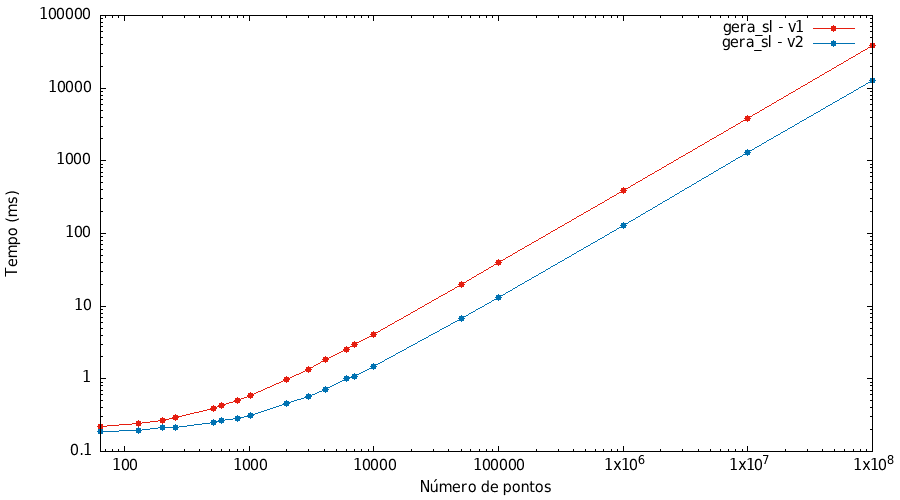
\includegraphics[width=\linewidth]{\path/tempo_gera_sl.png}
        \caption{Tempo de execução.}
        \label{gera_sl:tempo}
    \end{minipage}\hfill
    \begin{minipage}{.5\textwidth}
        \centering
        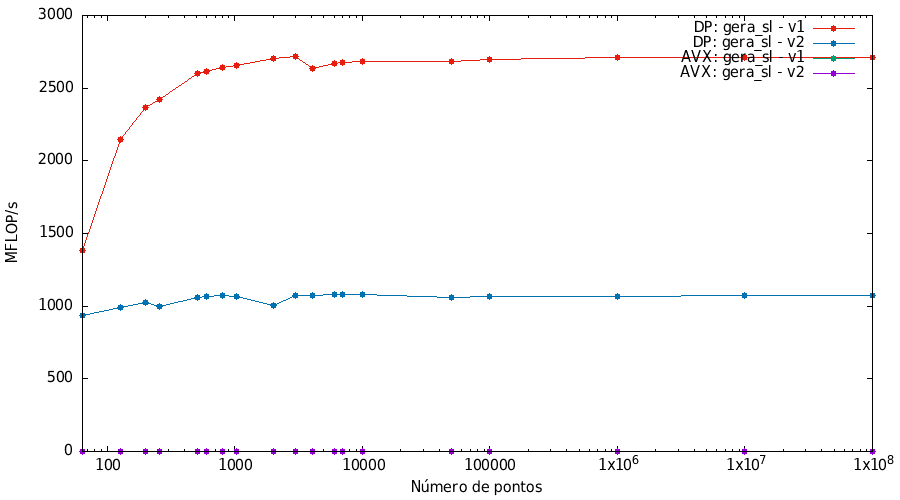
\includegraphics[width=\linewidth]{\path/operacoes_aritmeticas_gera_sl.png}
        \caption{Número de operações de ponto flutuante por segundo.}
        \label{gera_sl:flops}
    \end{minipage}
\end{figure}

Na figura \ref{gera_sl:tempo} o tempo da versão 2 é aproximadamente 4 vezes menor. Devido as otimizações de uso da \textit{cache} e cálculo da potência do intervalo.

Na figura \ref{gera_sl:flops} a quantidade de FLOP/s é muito maior na versão 1 devido ao uso da função \texttt{pow\_inter()}. A versão 2 tem menos FLOP/s devido ao reaproveitamento dos cálculos para exponenciação do intervalo.
%%\vspace{90pt} % precisamos de espaço aqui se nao os próximos gráficos não renderizam

\begin{figure}[H]
    \centering
    \begin{minipage}{.5\textwidth}
        \centering
        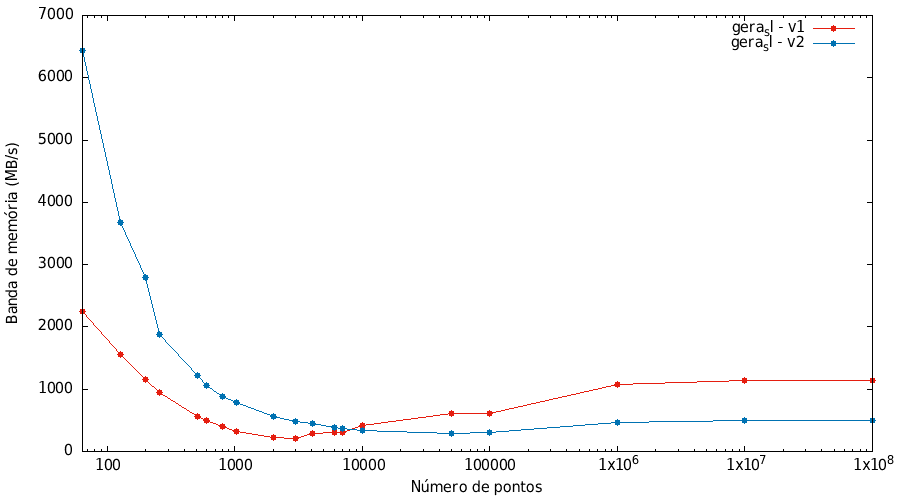
\includegraphics[width=\linewidth]{\path/banda_de_memoria_gera_sl.png}
        \caption{Banda de memória utilizada.}
        \label{gera_sl:banda}
    \end{minipage}\hfill
    \begin{minipage}{.5\textwidth}
        \centering
        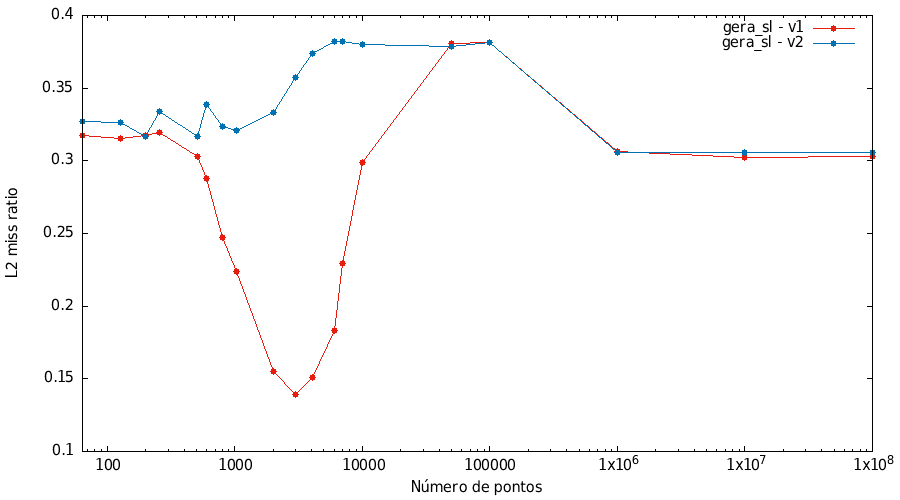
\includegraphics[width=\linewidth]{\path/cache_miss_l2_gera_sl.png}
        \caption{Taxa de \textit{miss} na \textit{cache} L2.}
        \label{gera_sl:cache_miss}
    \end{minipage}
\end{figure}

Na figura \ref{gera_sl:banda} a banda de memória é bem maior para um número pequeno de pontos devido a otimização que mantem os dados na \textit{cache}. Porém conforme o número de pontos vai aumentando as taxas vão diminuindo e se igualando, devido ao aumento de \textit{cache miss}.

Na figura \ref{gera_sl:cache_miss} o comportamento foi inesperado, devido as otimizações de uso da \textit{cache} o resultado esperado é que a versão 2 tenha um \textit{cache miss} menor que a versão 1.

\subsection{Solução do sistema linear}
\begin{figure}[H]
    \centering
    \begin{minipage}{.5\textwidth}
        \centering
        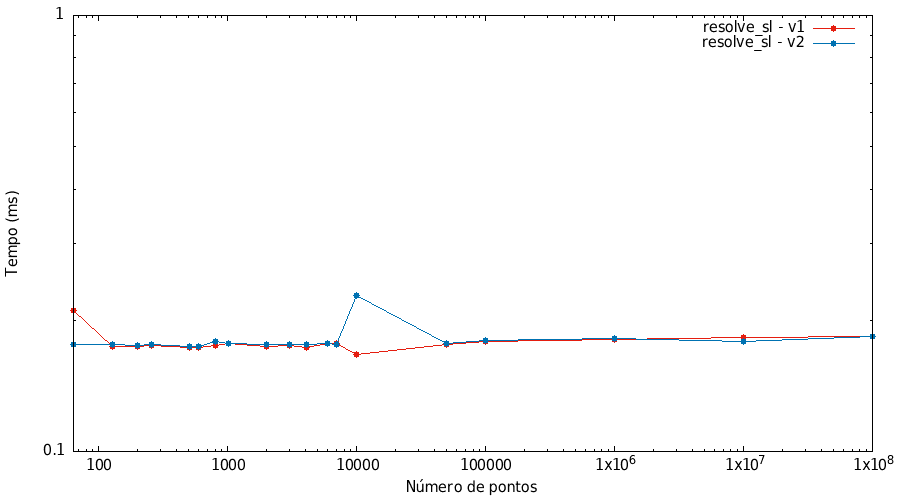
\includegraphics[width=\linewidth]{\path/tempo_resolve_sl.png}
        \caption{Tempo de execução.}
        \label{resolve_sl:tempo}
    \end{minipage}\hfill
    \begin{minipage}{.5\textwidth}
        \centering
        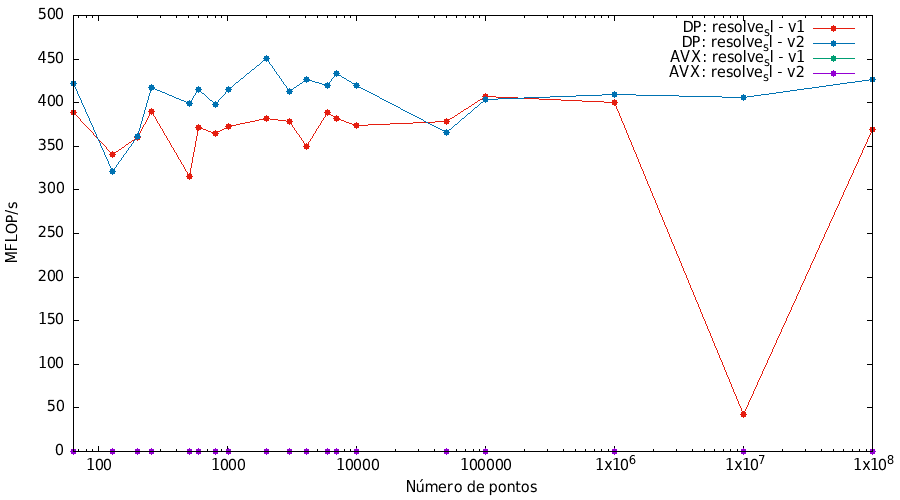
\includegraphics[width=\linewidth]{\path/operacoes_aritmeticas_resolve_sl.png}
        \caption{Número de operações de ponto flutuante por segundo.}
        \label{resolve_sl:flops}
    \end{minipage}
\end{figure}

Percebe-se pela figura \ref{resolve_sl:tempo} que o tempo de execução da
solução do sistema linear foi aproximadamente constante, indepentendemente
do número de pontos da entrada. Isso é devido ao fato de que a matriz sempre
possui ordem 5.

A figura \ref{resolve_sl:flops} apresenta uma constância independente do número de pontos e da versão, isso pois a matriz sempre possui ordem 5 e os cálculos não utilizam a função \texttt{pow\_inter()}.

\subsection{Cálculo de resíduos}
\begin{figure}[H]
    \centering
    \begin{minipage}{.5\textwidth}
        \centering
        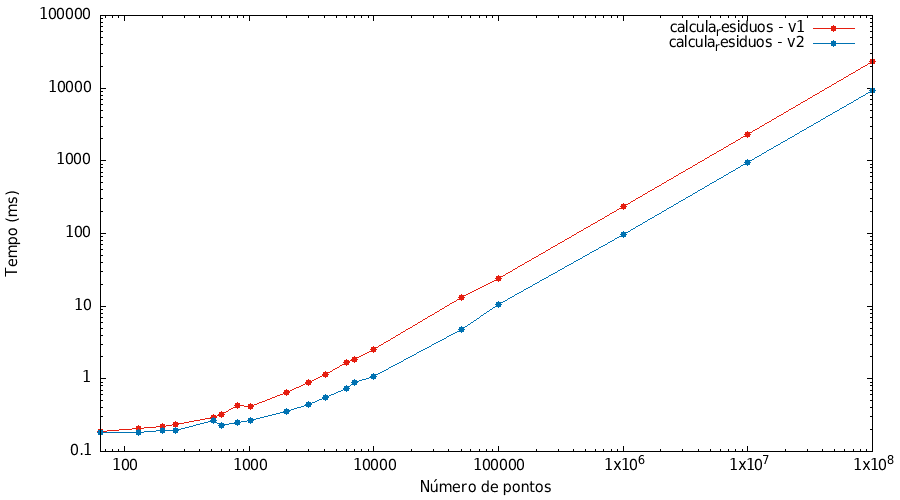
\includegraphics[width=\linewidth]{\path/tempo_calcula_residuos.png}
        \caption{Tempo de execução.}
        \label{calcula_residuos:tempo}
    \end{minipage}\hfill
    \begin{minipage}{.5\textwidth}
        \centering
        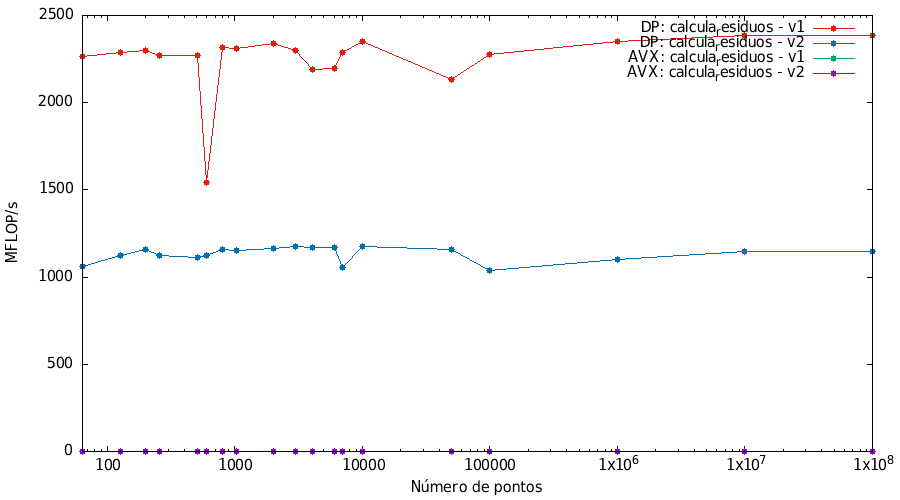
\includegraphics[width=\linewidth]{\path/operacoes_aritmeticas_calcula_residuos.png}
        \caption{Número de operações de ponto flutuante por segundo.}
        \label{calcula_residuos:flops}
    \end{minipage}
\end{figure}

A figura \ref{calcula_residuos:tempo} apresenta que o tempo de calcular os residuos é aproximadamente 4 vezes maior na versão 1 do que na versão 2, devido à otimização do uso da função \texttt{pow\_inter()}.

O número de FLOP/s é muito menor na versão 2, como pode ser visto na figura \ref{calcula_residuos:flops}. Isso pois a versão 2 otimiza o código e reaproeita a potência anterior de $x_i$ para calcular a nova potência, ao invés de utilizar a função \texttt{pow\_inter()}, que é custosa.

\begin{figure}[H]
    \centering
    \begin{minipage}{.5\textwidth}
        \centering
        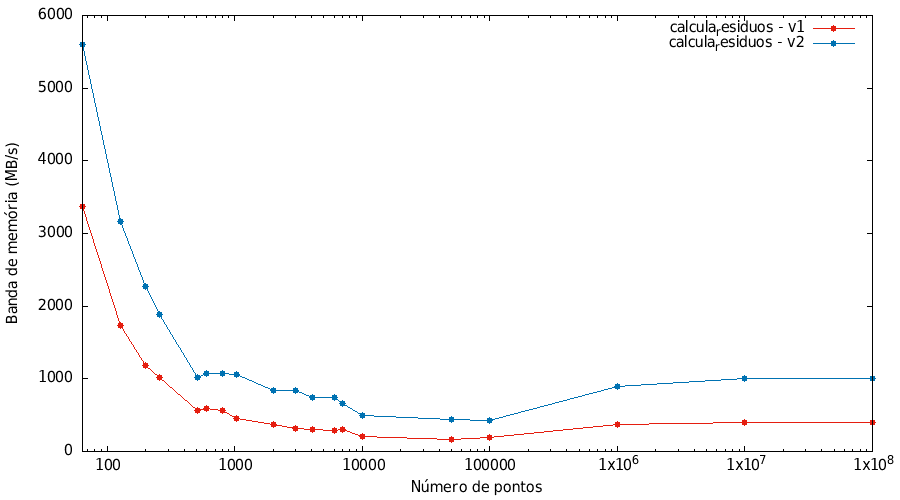
\includegraphics[width=\linewidth]{\path/banda_de_memoria_calcula_residuos.png}
        \caption{Banda de memória utilizada.}
        \label{calcula_residuos:banda}
    \end{minipage}\hfill
    \begin{minipage}{.5\textwidth}
        \centering
        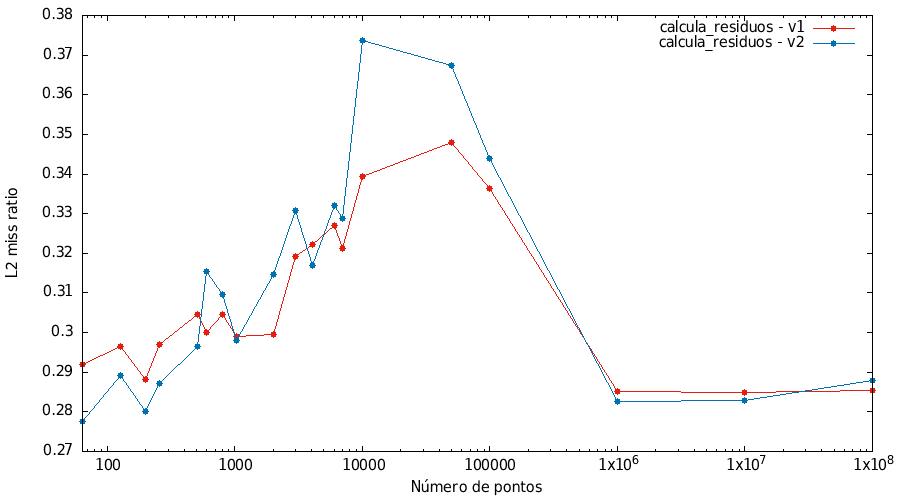
\includegraphics[width=\linewidth]{\path/cache_miss_l2_calcula_residuos.png}
        \caption{Taxa de \textit{miss} na \textit{cache} L2.}
        \label{calcula_residuos:cache_miss}
    \end{minipage}
\end{figure}

Em ambas as figuras \ref{calcula_residuos:cache_miss} e \ref{calcula_residuos:cache_miss} os valores são parecidos nas duas versões, isso pois a otimização no cálculo de resíduos foi na parte de operações aritméticas.

\end{document}
